\chapter{Software architecture}

% TODO: En este apartado empiezo a poner diagramas, los pongo a color o
% mejor en blanco y negro??

“Most systems work better they are kept simple rather than complicated”
\cite{kiss-wiki}. This is the main statement of the KISS principle, acronym for
“Keep it simple, stupid”. KISS philosophy is very used on software development
because code tends to chaos. If the implementation of a functionality is not
properly thought, it adds complexity to the program work flow. Therefore, to
reduce the architecture entropy is one of the main design patterns.

Model-View-Controller (MVC) is a well-known software architecture that consists
on the use of this tree elements to build a user interface. It was introduced 
by Trygve Reenskaug in the seventies \cite{mvc-past-present}. When web
applications appeared, this model was applied in many important projects
like \href{https://support.microsoft.com}{Microsoft Support}. 

% TODO: NO SE COMO PONER UNA WEB COMO EJEMPLO

\begin{figure}[htb]
	\begin{center}
		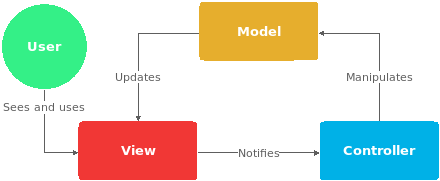
\includegraphics[width=0.5\textwidth]{./figures/mvc.png}
		\caption{Diagram of interactions within the MVC pattern.
				 \cite{mvc-wiki}}
		\label{F:mvc}
	\end{center}
\end{figure}

As shown on Figure \ref{F:mvc}, it is a simple model to represent
a user interface (UI). The UI visual representation is managed by the view.
Each time the user performs an action, view notifies controller and it modifies
the current model. Since view is watching it, the change is detected and view
is affected.

The problem is that this architecture becomes complex and complex while 
increasing the number of view. Actions from a view can affect other views'
model and this changes can trigger other actions. This complexity could even
generate unexpected loops as Figure \ref{F:mvc-complex} proves.

\begin{figure}[htb]
	\begin{center}
		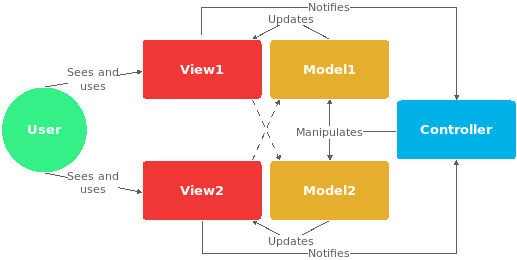
\includegraphics[width=0.6\textwidth]{./figures/mvc-complex.png}
		\caption{Diagram of interactions within the MVC pattern with many views}
		\label{F:mvc-complex}
	\end{center}
\end{figure}

\section{Flux-like architecture}

In order solve the MVC scalability problem, Facebook proposed Flux
\cite{flux-web}. Flux is the application architecture that Facebook uses for
building client-side web applications. To solve the loop problem, they devise
an “unidirectional data flow with changes described as plain objects”.

\begin{figure}[htb]
	\begin{center}
		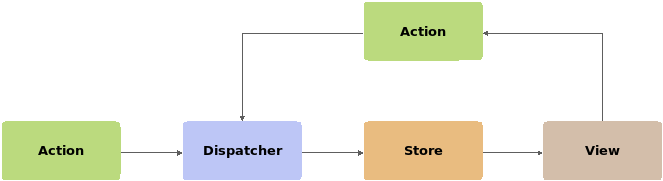
\includegraphics[width=0.7\textwidth]{./figures/flux.png}
		\caption{Diagram of Flux}
		\label{F:flux}
	\end{center}
\end{figure}

Even through Figure \ref{F:flux} appears to have a loop, with Flux things are
much easy to handle. View just wait change events produced by the store and
render themselves using the current state information. Note that render
processes do not need to call any action.

\subsection{React}

React is an implementation of Flux view piece. It is a component-based 
JavaScript library to build user interfaces \cite{react-web}. Each React
component can have input properties and a state, and must implement a render
function. Furthermore, to make things easier, React supports JSX which are
JavaScript files where HTML code can be used.


\begin{codefigure}
	\jsxexternal[
		caption=React hello world,
		label=L:react-hello-world,
		%
		classoffset=1,
		morekeywords={HelloMessage, React, Component, ReactDOM},
		classoffset=2,
		morekeywords={<HelloMessage},
	]{source/react-hello-world.jsx}
\end{codefigure}

Listing \ref{L:react-hello-world} shows up an example of React component. It has
a no state, a property call name and an easy render function to create a div.
Render functions can also have components inside themselves. That way, React
creates a component tree \ref{F:react-tree}.

\begin{figure}[htb]
	\begin{center}
		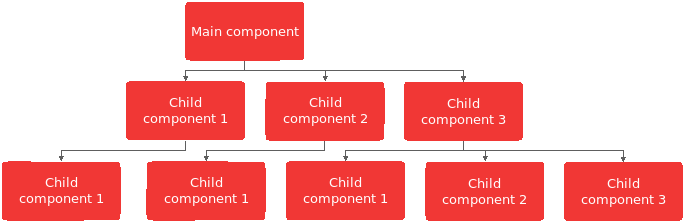
\includegraphics[width=0.7\textwidth]{./figures/react-tree.png}
		\caption{React tree}
		\label{F:react-tree}
	\end{center}
\end{figure}

Components may need to perform actions. Those cannot be performed on render 
function, as seen before. To do that, each component have a lifecyle. It 
consists of a functions' set that are called when some external actions happen. 
Most used ones are \textit{"componentWillMount"} and 
\textit{"componentWillUnmount"}. Components also can listen to its view
elements to perform actions.

\subsection{Redux}

Redux was inspired by several important qualities of Flux. Like Flux, Redux
prescribes that you concentrate your model update logic in a certain layer of
your application (“stores” in Flux, “reducers” in Redux) \cite{redux-prior-art}.
Redux have tree principles must be followed \cite{redux-principles}.

\begin{description}
	\item [Single source of truth]
	The state can be stored easily if just one store is used. Furthermore, the
	application will be easy to debug.
	
	\item [State is read-only]
	The only way to modify the state is using actions. Each time the state
	changes, a new state must be created.

	\item [Changes are made with pure functions]
	Reducers must be pure functions, that means, using the same initial state,
	repeating the same list of actions must produce the same final state.

\end{description}


\begin{figure}[htb]
	\begin{center}
		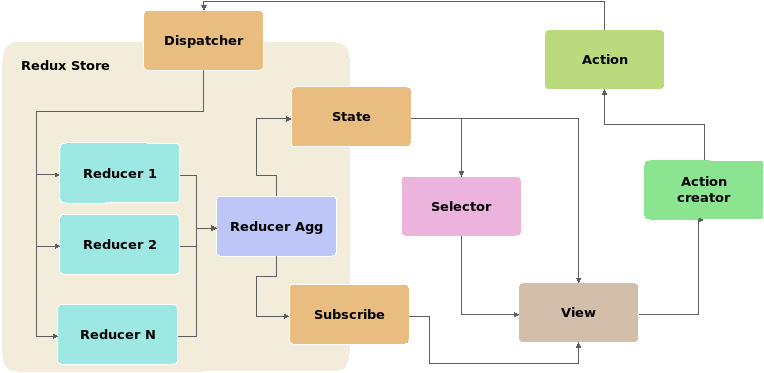
\includegraphics[width=0.8\textwidth]{./figures/redux.png}
		\caption{Redux architecture}
		\label{F:redux-architecture}
	\end{center}
\end{figure}

Figure \ref{F:redux-architecture} shows up the overall architecture of 
Redux. First of all a store must be created. This store contains reducers that
map action created by action creators into state changes. If needed, selectors
can be used to cache some state costly transformations. Store also exposes a
subscription function to receive state change notifications.

\subsubsection{Action creators}

An action is a plain JavaScript object that contains a field called type to 
identify it and other optional fields that are the payload. Same type of action
can be created in many places of the code so it is extremely recommended to use
action creators.

Action creators are functions that create those objects. Normally are defined
using lambdas. An example of action creator is shown on Listing
\ref{L:redux-action-creator}.

\begin{codefigure}
	\jsexternal[
		caption=Redux action creator,
		label=L:redux-action-creator,
	]{source/redux-action-creator.js}
\end{codefigure}

\subsubsection{Reducers}

Reducers aim to return new states each time an action is produced. They must be
implemented using pure functions. Tree statements must be followed.

The fist one is \textbf{mapping}. To fulfill it means that same input always 
returns the same output. Therefore, pure functions can not generate random
numbers nor current date. If this statement is not followed, functions are
difficult to test since its return value is unpredictable.

\begin{center}
	\textbf{KO}: \jsinline{ const mult = (x) => Math.random() * x; }
\end{center}

The way to fix this issue is simply adding this values as a parameter of the 
function.

\begin{center}
	\textbf{OK}: \jsinline{ const mult = (x, rnd) => rnd * x; }
\end{center}

The second statement is \textbf{Avoid side effects}. This means that function's
code must not modify anything that don't belong to it.

\begin{center}
	\textbf{KO}: \jsinline{ const title = (x) => document.title = x; }
\end{center}

Removing side effects makes the application's flow easy to follow reducing
complexity.

And last but not least \textbf{No external mutable}. This means that the output
of the function must be independent to changes once the value is retrieved. But
how can this happen? Easy, when a JavaScript object is assigned to another
variable, it is a reference, not a copy. If any of both variables changes, it
will affect also to the other. A simple example of this issue is shown on 
Listing \ref{L:obj-ref}.

\begin{codefigure}
	\jsexternal[
		caption=Object reference effect,
		label=L:obj-ref,
	]{source/obj-ref.js}
\end{codefigure}

Therefore, an example of non pure function due to no external mutation is:

\begin{center}
	\textbf{KO}: \jsinline{ const rename = (obj, val) => obj.name = val; }
\end{center}

The way to make this function follow no external mutable principle, the returned
object must be a copy for the one provided as parameter.

\begin{center}
	\textbf{OK}: \jsinline{
		const rename = (obj, val) => \{ ...obj, name: val \};
	}
\end{center}

Then applying this three principles, Listing \ref{L:redux-reducer} shows up an
example of reducer for action shown on Listing \ref{L:redux-action-creator}.

\begin{codefigure}
	\jsexternal[
		caption=Redux reducer,
		label=L:redux-reducer,
	]{source/redux-reducer.js}
\end{codefigure}

This function in called by the store each time an action is dispatched. 
Reducers can be aggregated using a function provided by Redux called
\textit{"combineReducers"}. Listing \ref{L:redux-agg-reducers} shows an example.

\begin{codefigure}
	\jsexternal[
		caption=Reducer aggregation,
		label=L:redux-agg-reducers,
	]{source/redux-agg-reducers.js}
\end{codefigure}

\subsubsection{Selectors}
\label{S:selectors}

Selectors are pure functions that can cache the return value and it is just 
recomputed if any of the input parameters changes. For instance, a selector
can be created to select items that starts with letter 'I'. This example is
shown on Listing \ref{L:redux-selector}.

\begin{codefigure}
	\jsexternal[
		caption=Redux selector,
		label=L:redux-selector,
	]{source/redux-selector.js}
\end{codefigure}

\subsubsection{Store}

To create a store is as easy as provide the root reducer and the initial state.
Then actions can be dispatched and a function can be subscribed to detect any
state change.

Listing \ref{L:redux-store} shows how to create a store. Also,
selector created in Section \ref{S:selectors} is used to calculate the items'
subset just if they have change. Also, several actions are dispatched.

\begin{codefigure}
	\jsexternal[
		caption=Redux store creation and management,
		label=L:redux-store,
	]{source/redux-store.js}
\end{codefigure}

\subsection{Action observables}

Observables are data streams provided by a library called Reactive Extensions
for JavaScript (rxjs). The idea is to treat those streams as asynchronous 
events and apply fluent query operators.

\begin{codefigure}
	\jsexternal[
		caption=Rxjs observable to count seconds until last click,
		label=L:rxjs-simple-observable,
	]{source/rxjs-simple-observable.js}
\end{codefigure}

As shown on Listing \ref{L:rxjs-simple-observable}, complex behaviors can be
implemented in an easy to read way using this library. The example shows up
how to count the difference in time between two button clicks. To do that, 
an observable is created to watch the event click of a button. The operator scan
caches the last returned value sending it as first parameter of the callback
function. Last scanned is mapped to get the difference in seconds of last
and current time values. Finally, this difference is printed on a text element.

Since Redux's reducers must be pure functions and there are many complex
behaviors that have to be chained when some actions are produced, Redux
Observables provides a middleware that handles action streams using rxjs
observables. The observable is executed after the action has been reduced.
So Redux architecture (Figure \ref{F:redux-architecture}) must be complemented 
with Figure \ref{F:redux-observables-architecture}.

\begin{figure}[htb]
	\begin{center}
		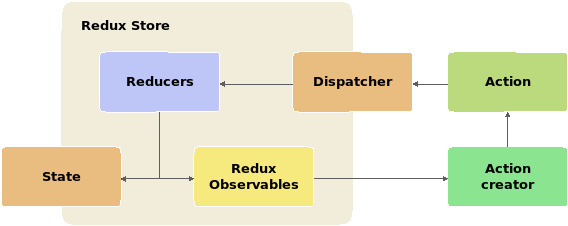
\includegraphics[width=0.6\textwidth]{./figures/redux-observables.png}
		\caption{Redux Observables architecture}
		\label{F:redux-observables-architecture}
	\end{center}
\end{figure}

\subsection{React-Redux}

To let React and Redux work together, Redux store must be provided inside React
tree. Also, action creators and state have to be mapped into React properties.

\begin{landscape}
\begin{figure}[htp]
	\begin{center}
		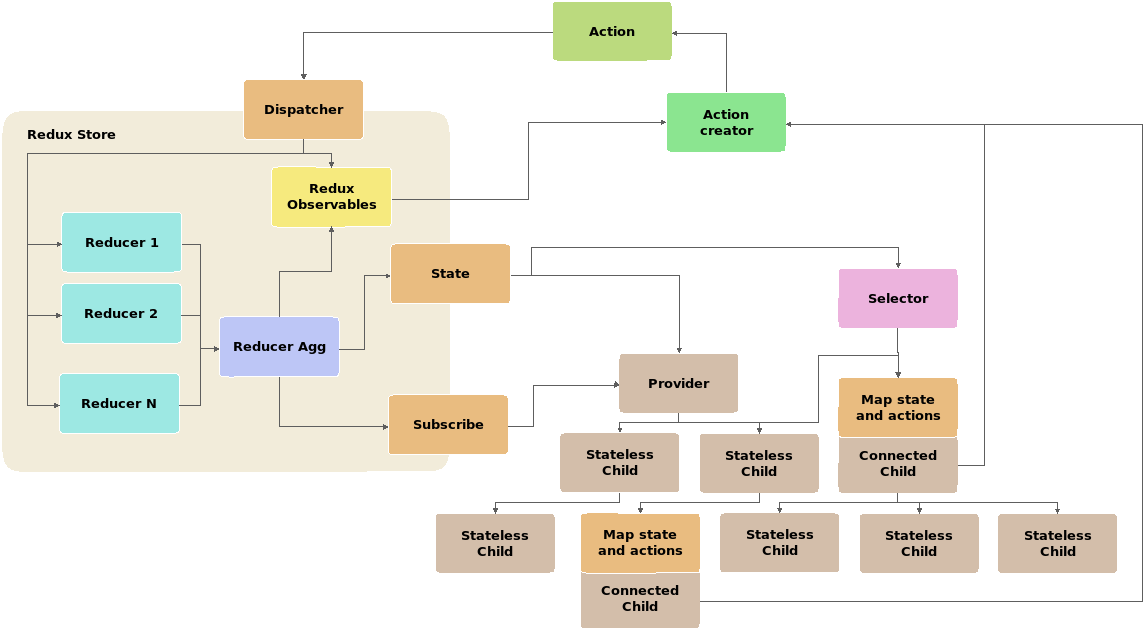
\includegraphics[width=1.3\textwidth]
		{./figures/overall-architecture.png}

		\caption{Overall architecture}
		\label{F:overall-architecture}
	\end{center}
\end{figure}
\end{landscape}

\section{The Sleuth Kit JavaScript}



